\section{Design and Methodology}

\subsection{Data Collection}
The data was collected using the Twitter Streaming API between October 2017 and September 2018. A location filter was specified so that only tweets posted from within the bounding box of Dublin were returned. 2.5 million tweets were collected.

We discovered that a significant number of tweets had slipped through Twitter's location filter. This meant that the first step required was to filter the dataset to ensure, as much as was possible, that all tweets related to Dublin.

\subsection{Data Filtering}

\subsubsection{Filtering Out Non-Dublin Tweets}
All of the tweets were Geo-tagged because they were collected with Twitter's location filter. There are two types of Geo-tagged tweets, tweets with a 'Point Coordinate' (a specific latitude/longitude), and tweets with a 'Twitter Place' (a bounding box defining a general place). Only 7.23\% of the tweets had point coordinates so a combination of Twitter place and point coordinates was used to filter out any non-Dublin tweets. A bounding box for the Dublin area was defined (North Latitude: 53.425210, South Latitude: 53.223430, East Longitude: -6.043924, West Longitude: -6.447485). Each tweet with a point coordinate was checked to see if the point fell within the Dublin's bounding box. If it lay inside the box it was kept, otherwise, it was filtered out. The centroid of the bounding box of each tweet with a Twitter place was calculated and checked to see if it fell within Dublin's bounding box. If it lay inside the box it was kept, otherwise, it was filtered out. The filtered dataset consisted of 1.6 million tweets.

\subsubsection{Filtering Tweets About Hotels}
A list of the hotels in Dublin was compiled. This included the hotel's names and Twitter handles. This list consisted of 159 hotels and Twitter handles. The tweets were stored in a Lucene index and a fuzzy search query was used to match the tweets against each of the hotel names and hotel Twitter handles. The fuzzy search query uses a similarity measure that is based on the Damerau-Levenshtein algorithm. The maximum edits option was set to two, meaning that strings with a maximum difference of two characters would still match. This accounted for misspellings and broadened our search slightly. We experimented with higher numbers of maximum edits but found that too many irrelevant tweets were returned. This further filtered dataset consisted of 3115 tweets that mention hotels posted from Dublin.

\subsection{Dataset Annotation}

In order to train a classifier to categorise the tweets as review-like tweets, tweets that contain some content and irrelevant tweets, a set of tweets had to first be manually annotated. The 3115 tweets about hotels in Dublin were annotated. This involved building an annotation webpage where users could view tweets and assign them labels (Figure ~\ref{fig:webpage}).

\begin{figure}[h!]
\centering
\fbox{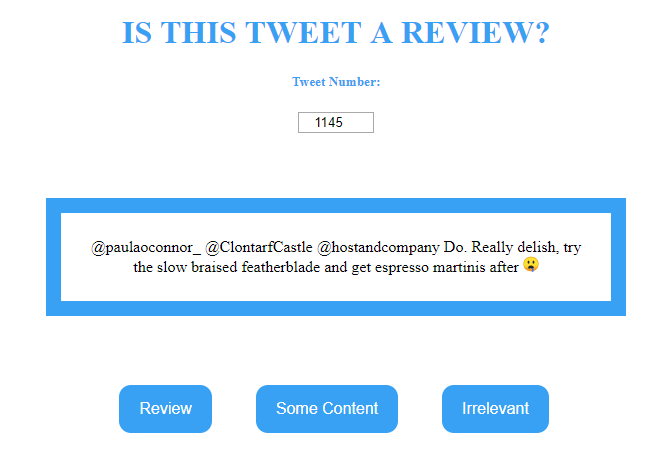
\includegraphics[width=0.95\columnwidth]{design_and_methodology/webpage.PNG}}
\caption{\label{fig:webpage} Tweet Annotation Webpage.}
\end{figure}

The text of each tweet was displayed alongside three buttons: 'Review', 'Some Content' and 'Irrelevant'. The participant could click on the option that they thought best described the tweet shown. 

The following instructions, describing what a 'Review', 'Some Content' and 'Irrelevant' tweet should look like accompanied the webpage:
\begin{itemize}
    \item Review: The tweet could be considered as a review (of any aspects related to a hotel such as the venue, food, view, swimming pool, etc.) for any hotel.
    \item Some Content: The tweet doesn't look like a review, but it does provide some information related to a hotel, such as the hotel hosts events, information on the menu, information related to accommodation, etc. 
    \item Irrelevant: This tweet is completely irrelevant. While perhaps mentioning the name of a hotel, the tweet doesn't give any additional information about that hotel or offer any opinions related to the hotel.
\end{itemize}

In this research, we decided to focus solely on the text of the tweets. For this reason, all images, videos and URLs were stripped from the tweets before being displayed on the annotation webpage. Images, videos and URLs could all carry valuable information and could be considered in future research. 

\subsection{Tweet Classification}
The annotated set of tweets was used to train thirteen classifiers with seven feature representations to determine which combination was most suited to the task. These classifiers were implemented using Python's Scikit Learn library \cite{scikit-learn}. The data was split 80:20 into a training set and a testing set.

\subsubsection{Data Pre-processing}

The following steps were taken to pre-process the tweets before they were used to train the classifiers:
\begin{itemize}
    \item Emojis were removed and replaced with text using Python's Emoji library \cite{emoji}.
    \item Special characters and punctuation were removed from the tweets. 
    \item All single characters were removed.
    \item Words were split on case changes.
    \item Words were split on word-digit boundaries.
    \item All text was converted to lower case.
    \item Stemming was performed using the Word Net Lemmatizer from the Natural Language Toolkit (\url{https://www.nltk.org/}.
    \item Stop words were removed in some cases using Scikit Learn's English stop word list. It will be clearly stated in all cases where stop words were removed.
\end{itemize}

\subsubsection{Feature Representation}

Seven feature extraction methods were implemented to see which performed best:
\begin{itemize}
    \item Unigram Bag-of-Words (BOW): A unigram implementation of BOW. In BOW documents are described by word occurrences. A tweet is represented as a feature vector consisting of ones and zeroes. One representing a term's occurrence and zero representing a term's absence.
    \item Unigram TF-IDF: A unigram implementation of TF-IDF. BOW can be extended with TF-IDF (Term Frequency-Inverse Document Frequency). The idea of TF-IDF is to balance how important a term is in a document versus how important it is in the entire collection. TF-IDF is used to re-weight the features produced by BOW.
    \item Bigram TF-IDF: A bigram implementation of TF-IDF. Another extension of BOW is the use of N-grams. An N-gram is a sequence of N consecutive terms. Combining bigrams with BOW means that occurrences of pairs of words are counted instead of individual terms.
    \item Trigram TF-IDF: A trigram implementation of TF-IDF.
    \item Unigram TF-IDF (stop words removed): A unigram implementation of TF-IDF with stop words removed.
    \item Word2Vec: Gensim's implementation of word2vec with Google's pretrained model. Word2Vec takes a dataset as its input and produces a vector space, where each word is represented by a corresponding vector.
    \item Doc2Vec: Gensim's implementation of doc2vec, with each tweet being considered a document. Doc2Vec takes a dataset as its input and produces a vector space, where each document is represented by a corresponding vector. Unlike Word2Vec, we built our own Doc2Vec vocabulary based on the training data.
\end{itemize}

\subsubsection{Classification Algorithms}
The annotated set of tweets was used to train a series of thirteen different classifiers to determine which classifier was most suited to the task. Each classifier was implemented with it's implementation from Python's Scikit Learn library \cite{scikit-learn}:
\begin{itemize}
    \item Decision Tree (DT): DT learns simple decision rules based on the training data. These decision rules form a tree structure which is used to predict the value of a target variable.
    \item Random Forest (RF): RF is an ensemble method. It combines multiple DT classifiers. The final class prediction is calculated by getting the average of the decisions of the individual DTs.
    \item Multi Layer Perceptron (MLP): MLP is a feedforward, artificial neural network. It consists of a minimum of three layers: an input layer, a hidden layer and an output layer. The input layer receives the data, the output layer makes a decision and the hidden layers approximate the function.
    \item Logistic Regression (LR): LR uses the logistic function to model the training data. 
    \item Support Vector Machine (SVM): SVM finds the optimum hyperplane that separates the data into the labelled classes. It aims to maximise the distance between the hyperplane and the support vectors.
    \item K Nearest Neighbours (KNN): KNN assigns a label to a document based on the class that has the majority of "nearest neighbours" to the document.
    \item Gaussian Process (GP): GP implements Gaussian Processes for classification. Gaussian Processes are probability distributions over possible functions.
    \item AdaBoost (AB): AB fits a series of weak base classifiers on incrementally re-weighted versions of the training data.
    \item Gaussian Naive Bayes (GNB): GNB is one of a set of Naive Bayes (NB) Classification algorithms. All of the NB classifiers apply Bayes Rule along with the ‘naive’ assumption that features are conditionally independent.
    \item Bernoulli Naive Bayes (BNB): BNB implements the NB algorithm for data that is distributed according to multivariate Bernoulli distributions.
    \item Multinomial Naive Bayes (MNB): MNB implements the NB algorithm for multinomial distributed data.
    \item Quadratic Discriminant Analysis (QDA) and Linear Discriminant Analysis (LDA): QDA and LDA, have quadratic and linear decision surfaces, respectively.
\end{itemize}

\subsection{Sentiment Analysis}

The Stanford NLP Sentiment Analyser \cite{stanfordSentiment2013} was used to classify the sentiment of the tweets. It was chosen as it is the dominant NLP library used in research in this area. The Sentiment Analyser classifies the text as Very Negative, Negative, Neutral, Positive or Very Positive. It also provides a sentiment distribution which shows how strongly the tweet aligns with each class. The scores produced by the Sentiment Analyser were produced per tweet.

A majority voting technique was used to normalise the scores. For each hotel, we had a selection of tweets. These tweets are divided into five clusters: very negative, negative, neutral (ignored), positive and very positive. A mean value was calculated for each cluster, by summing the corresponding score in the sentiment distribution for each tweet and dividing by the number of tweets in the cluster. The class with the highest mean value was assigned to the hotel. This mean score was then normalised between zero and one using max-min normalisation, with the following weighting: 
\begin{itemize}
    \item Very Negative: 0 - 0.25
    \item Negative: 0.25 - 0.5
    \item Positive: 0.5 - 0.75
    \item Very Positive: 0.75 - 1
\end{itemize}

%These max-min normalisation formulae were used to calculate the normalised scores (NS):
%\begin{equation}
%\setlength{\abovedisplayskip}{3pt}
%\setlength{\belowdisplayskip}{0pt}
%\resizebox{.8\linewidth}{!}{NS (-) = max\ score-(actual\ score \times (max\ score - min\ score))}    
%\end{equation}

%\begin{equation}
%\setlength{\abovedisplayskip}{0pt}
%\setlength{\belowdisplayskip}{0pt}
%\resizebox{.8\linewidth}{!}{NS (+) = (actual\ score \times (max\ score - min\ score)) + min\ score}
%\end{equation}

\subsection{CoRE Recommender System}

CoRE \cite{core2019} is a Cold Start Resistant and Extensible Recommender system. The CoRE recommender is an algorithmic approach to hotel recommendation, that makes use of collaborative filtering, content-based recommendation and contextual suggestion. It is made up of three models, a user model, a segment model and a context model. Each model is generated as a weighted feature vector and combined by calculating the centroid vector. A weighting is applied to determine the effect of each model in the final vector. The cosine similarity between the vector of each hotel and the centroid vector of the user is then calculated, and a list of hotels is produced. The hotels are ranked based on the similarity score. CoRE was evaluated against the ranking approach currently used by Ryanair. In this approach hotels from the target city are sorted based on their transactional data from the last 30 days. CoRE significantly outperforms this baseline.

The sentiment scores produced by the Stanford NLP Sentiment Analyser were used to re-rank the list of hotel recommendations produced by CoRE. This was done by multiplying the score of the hotel in the CoRE ranked list by the normalised sentiment score. This boosts the score of hotels with a positive sentiment score and drags down the score of the hotels with a negative sentiment score.